\documentclass[tikz,border=4pt]{standalone}
% Shared TikZ style for lecture figures
\usepackage{amsmath,amssymb}
\usepackage{tikz}
\usetikzlibrary{arrows.meta,calc,decorations.pathreplacing,patterns}
\definecolor{teal}{RGB}{38,150,140}
\definecolor{coral}{RGB}{230,95,75}
\definecolor{ink}{RGB}{20,45,60}
\tikzset{
  >={Stealth[length=2.6mm]},
  every picture/.style={line cap=round,line join=round,thick,ink},
  map/.style={->,thick},
  dot/.style={circle,fill,inner sep=1.2pt},
}

\begin{document}
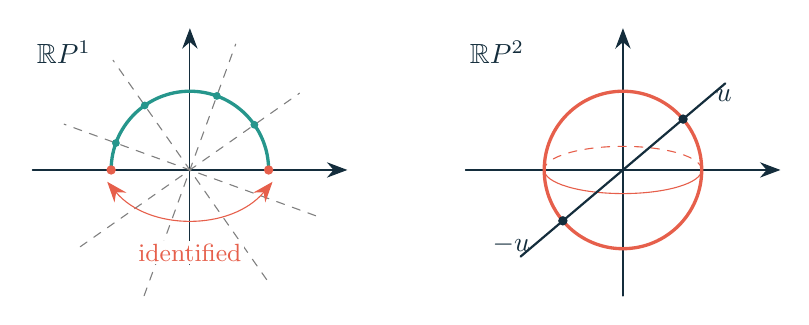
\begin{tikzpicture}
  % RP^1
  \draw[->,thin] (-2,0) -- (2,0);
  \draw[->,thin] (0,-1.2) -- (0,1.8);
  \foreach \a in {35,70,125,160}{
    \draw[gray,thin,dashed] ({-1.7*cos(\a)},{-1.7*sin(\a)}) -- ({1.7*cos(\a)},{1.7*sin(\a)});
    \node[dot,teal,inner sep=1pt] at ({cos(\a)},{sin(\a)}) {};
  }
  \draw[teal,very thick] (1,0) arc (0:180:1);
  \node[dot,coral] at (1,0) {};
  \node[dot,coral] at (-1,0) {};
  \draw[coral,<->,thin] (-1.05,-0.15) to[bend right=50] (1.05,-0.15);
  \node[coral,fill=white,inner sep=1pt] at (0,-1.05) {\small identified};
  \node at (-1.6,1.5) {$\mathbb{R}P^{1}$};
  % RP^2
  \begin{scope}[xshift=5.5cm]
    \draw[->,thin] (-2,0) -- (2,0);
    \draw[->,thin] (0,-1.6) -- (0,1.8);
    \draw[coral,very thick] (0,0) circle (1);
    \draw[coral,thin] (1,0) arc (0:-180:1 and 0.3);
    \draw[coral,thin,dashed] (1,0) arc (0:180:1 and 0.3);
    \draw[thick] (-1.3,-1.1) -- (1.3,1.1);
    \node[dot] at ({cos(40.24)},{sin(40.24)}) {};
    \node[dot] at ({-cos(40.24)},{-sin(40.24)}) {};
    \node at (1.05,0.95) [right] {$u$};
    \node at (-1.05,-0.95) [left] {$-u$};
    \node at (-1.6,1.5) {$\mathbb{R}P^{2}$};
  \end{scope}
\end{tikzpicture}
\end{document}
